% ===================================================================
%  Αρχείο: 15372_tikz.tex (Fragment)
%  Αυτόματη μετατροπή μέσω doc2latex.py & TikZ conversion
% ===================================================================

ΘΕΜΑ 2

\begin{center}
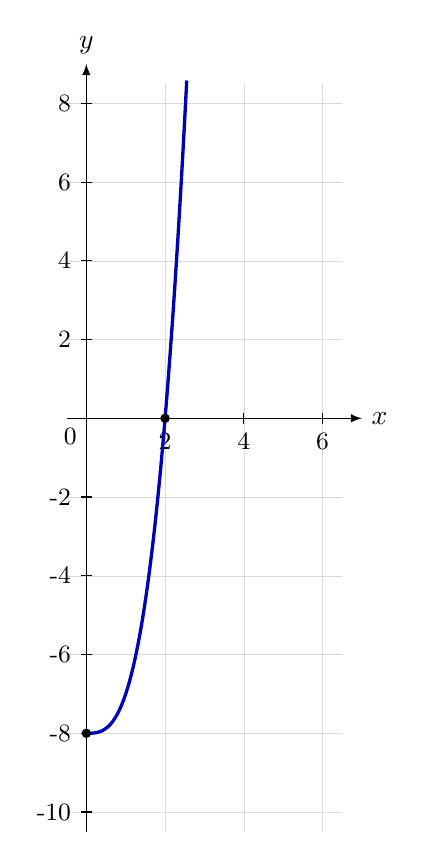
\begin{tikzpicture}[scale=0.5, >=latex]
    \draw[very thin, color=gray!30, step=2] (-0.5,-10.5) grid (6.5,8.5);
    \draw[->] (-0.5,0) -- (7,0) node[right] {$x$};
    \draw[->] (0,-10.5) -- (0,9) node[above] {$y$};
    
    \foreach \x in {2,4,6}
        \draw (\x,4pt) -- (\x,-4pt) node[below, font=\small] {\x};
    \foreach \y in {-10,-8,-6,-4,-2, 2,4,6,8}
        \draw (4pt,\y) -- (-4pt,\y) node[left, font=\small] {\y};
    \node[below left, font=\small] at (0,0) {$0$};
    
    % Curve passing through (0,-8) and (2,0)
    % Roughly y = x^3 - 8 for x > 0
    \draw[very thick, color=blue!70!black, samples=100, smooth, domain=0:2.55] plot (\x, {\x*\x*\x - 8});
    
    \filldraw (0,-8) circle (3pt);
    \filldraw (2,0) circle (3pt);
\end{tikzpicture}
\end{center}

Στο παραπάνω σχήμα δίνεται ένα τμήμα της γραφικής παράστασης μιας άρτιας συνάρτησης με πεδίο ορισμού το$\ \mathbb{R.}$

\begin{alist}
\item Να μεταφέρεται το σχήμα στην κόλλα σας και να συμπληρώσετε τη γραφική παράσταση με το κομμάτι της καμπύλης που λείπει. Να αιτιολογήσετε την απάντησής σας.

\monades{10}

\item Να βρείτε:
\begin{rlist}
\item Τα διαστήματα μονοτονίας της συνάρτησης f.

\monades{8}

\item Tο είδος του ακροτάτου και τη θέση που το παρουσιάζει.

\monades{7}
\end{rlist}
\end{alist}
